% !TeX root = ../main.tex

\chapter{基于事件相机的火焰数据集构建}
在之前绪论的火焰数据集部分,本文已经提到目前领域内常用的数据集以可见光相机拍摄为主,缺乏效果优秀的、公开的基于事件相机的火焰数据集,本章中将使用DAVIS346事件相机收集相关的火焰数据并着手制作一个初步的火焰检测数据集,称之为 \textbf{Fla}me \textbf{D}etection based on \textbf{E}vent dataset,后面统一用FlaDE指代该数据集。

\section{火焰数据集}
火焰检测数据集和其他的目标检测相似,也分为图像与视频两个大类,分别用于静态与动态不同的检测算法
训练与测试。例如著名的Dyntex公开库\cite{peteri2008comprehensive}中,提供了数百个动态视频纹理系列,其中的每个序列时间大于十秒,一秒25帧,
均为720x576的图像,同时每个均备注了一些相关的信息,包括采集的时间,设备,环境条件等。这里值得提及的是,视频数据集作为训练动态算法的连续帧视频文件,其帧数可以有所不同,由几秒到几分钟不等,但是往往
需要包含有火和无火两类场景,不同的环境条件,例如光照、风况,也均会对其效果造成不小影响。

同时目前也出现了大量的火焰烟雾场景为主的数据集,期望能够对早期烟雾进行检测识别而更早确定火灾场景。这里再以MIVIA数据集\cite{foggia2015real}为例,它分火焰集与烟雾集,包含的
火灾集视频序列共31个,分别是17个无火焰视频和14个火灾场景,均为不同环境拍摄,分类较为细致。同时它的烟雾集设置了很多远镜头烟雾场景,内含天空、云、强自然光等干扰,很考验
待测算法的准确度。此外还有中国科学技术大学火灾科学国家实验室制作的烟雾数据集,已经过人工标注,其中包含上万张的烟雾与非烟雾图像,包括真实烟雾与合成烟雾,
可以有效胜任深度网络训练。

\section{FlaDE检测数据集}
为研究火焰在事件领域的特征分布和设计火焰检测算法,本文制作了一套基于事件相机的火焰检测数据集,称之为FlaDE。该数据集由型号为DAVIS346的事件相机进行拍摄制作,该相机以$346\times260$的空间分辨率和\SI{1}{\micro\second}的时间分辨率输出事件数据(动态范围\SI{120}{\decibel}),输出带宽可达12MEPS。此外,该相机还能以最大40fps的帧率输出时间同步的灰度图像(动态范围\SI{56.7}{\decibel}),并内置6轴惯性测量单元(采样率\SI{8}{\kilo\hertz})记录设备的角速度和加速度。

数据集拍摄场景选取在一片具有植被覆盖的开阔场地中,拍摄开始前,一个木垛火将被点燃,随即打开事件相机进行数据录制。拍摄过程中,相机被固定在三脚架上进行记录,并在整个数据采集期间始终保持静止。考虑到算法在不同监控视角下的适用性,这里选取有明显区别的拍摄角度和距离对火焰进行捕捉,并剪切成不同的数据片段,其中一个数据片段如图\ref{subfig:FlaDE_01}所示。

事件相机对光线变化的高灵敏度虽然提供了优越的捕捉能力,但也带来了挑战,尤其是在复杂光照条件下的噪声问题。为此,本文特别录制了一系列夜间场景,在这些场景中,事件数据将伴随有大量的噪声信号,从而干扰火焰检测算法的性能(图\ref{subfig:FlaDE_02})。同时本文也测试了一些传统相机可能遇到的特殊情况,例如图像过曝(图\ref{subfig:FlaDE_03})和物体遮挡(图\ref{subfig:FlaDE_04}),以此检验事件相机在火焰检测中相对于传统相机来说是否具有特殊优势。上述数据片段的设置对火焰检测算法的鲁棒性提出了更高的要求。

\begin{figure}[ht]
    \centering
    \begin{subfigure}{0.32\textwidth}
        \centering
        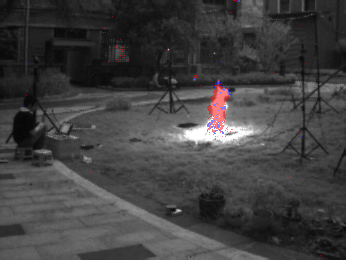
\includegraphics[width=\textwidth]{figures/FlaDE_01.png}
        \caption{F01\textunderscore c02\textunderscore 00285}
        \label{subfig:FlaDE_01}
    \end{subfigure}
    \hfill
    \begin{subfigure}{0.32\textwidth}
        \centering
        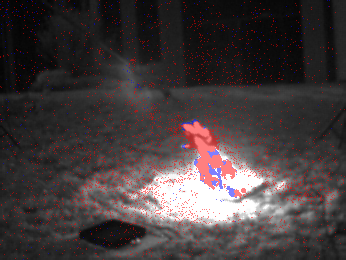
\includegraphics[width=\textwidth]{figures/FlaDE_02.png}
        \caption{F01\textunderscore c05\textunderscore 00191}
        \label{subfig:FlaDE_02}
    \end{subfigure}
    \hfill
    \begin{subfigure}{0.32\textwidth}
        \centering
        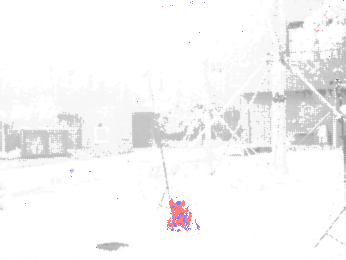
\includegraphics[width=\textwidth]{figures/FlaDE_03.png}
        \caption{F02\textunderscore c02\textunderscore 00502}
        \label{subfig:FlaDE_03}
    \end{subfigure}
    % 
    \begin{subfigure}{0.32\textwidth}
        \centering
        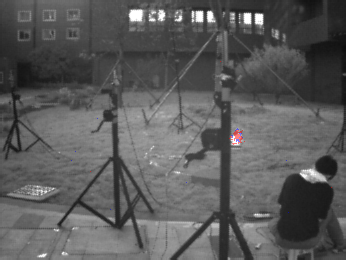
\includegraphics[width=\textwidth]{figures/FlaDE_04.png}
        \caption{F02\textunderscore c04\textunderscore 00296}
        \label{subfig:FlaDE_04}
    \end{subfigure}
    \hfill
    \begin{subfigure}{0.32\textwidth}
        \centering
        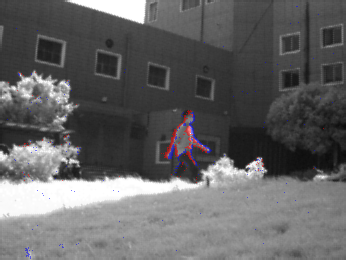
\includegraphics[width=\textwidth]{figures/FlaDE_05.png}
        \caption{P02\textunderscore c02\textunderscore 00408}
        \label{subfig:FlaDE_06}
    \end{subfigure}
    \hfill
    \begin{subfigure}{0.32\textwidth}
        \centering
        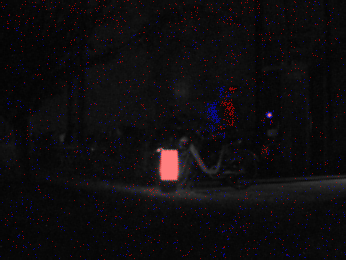
\includegraphics[width=\textwidth]{figures/FlaDE_06.png}
        \caption{L01\textunderscore c01\textunderscore 00598}
        \label{subfig:FlaDE_05}
    \end{subfigure}
    %
    \caption{FlaDE数据集片段}
\end{figure}

此外,本文特意录制了包含常见干扰物(行人、灯光闪烁)的场景,如图\ref{subfig:FlaDE_05}和图\ref{subfig:FlaDE_06}所示。通过引入非火焰动态场景构建数据集的负样本集,有助于后续评估算法在误报率方面的表现。

最终的数据集包含10444个包含单火焰的序列作为正样本、7144个行人和3228个灯光的序列作为负样本补充。

\section{数据集预处理}
火焰检测数据集需要真实标签数据作为参考结果来与检测算法所预测的标签数据进行对比,因此本文为FlaDE数据集制作了真实的数据标签。注意到由于事件数据是存在于时间-空间领域中的四元组,因此需要对其进行预处理,以方便标注工作的进行,具体流程如下:

步骤一:采用RED递归去噪算法\cite{ding2023}对事件数据的噪声进行滤除(\ref{subfig:FlaDE_denoising})。RED算法通过设计空间高斯核函数和时间高斯核函数进行逐事件的核密度估计,从而有效的滤除噪声,其中去噪参数(空间方差$\sigma_s$和时间方差$\sigma_t$)由人手动进行调整以达到最优的去噪结果。处理过程中采用该算法的DV版本\footnote{https://docs.inivation.com/}进行逐序列的手动调节,以确保尽可能多地抑制噪声,保留有效事件,同时本文也提供了具有挑战性的非去噪版本。

\begin{figure}[ht]
    \centering
    \begin{subfigure}{0.49\textwidth}
        \centering
        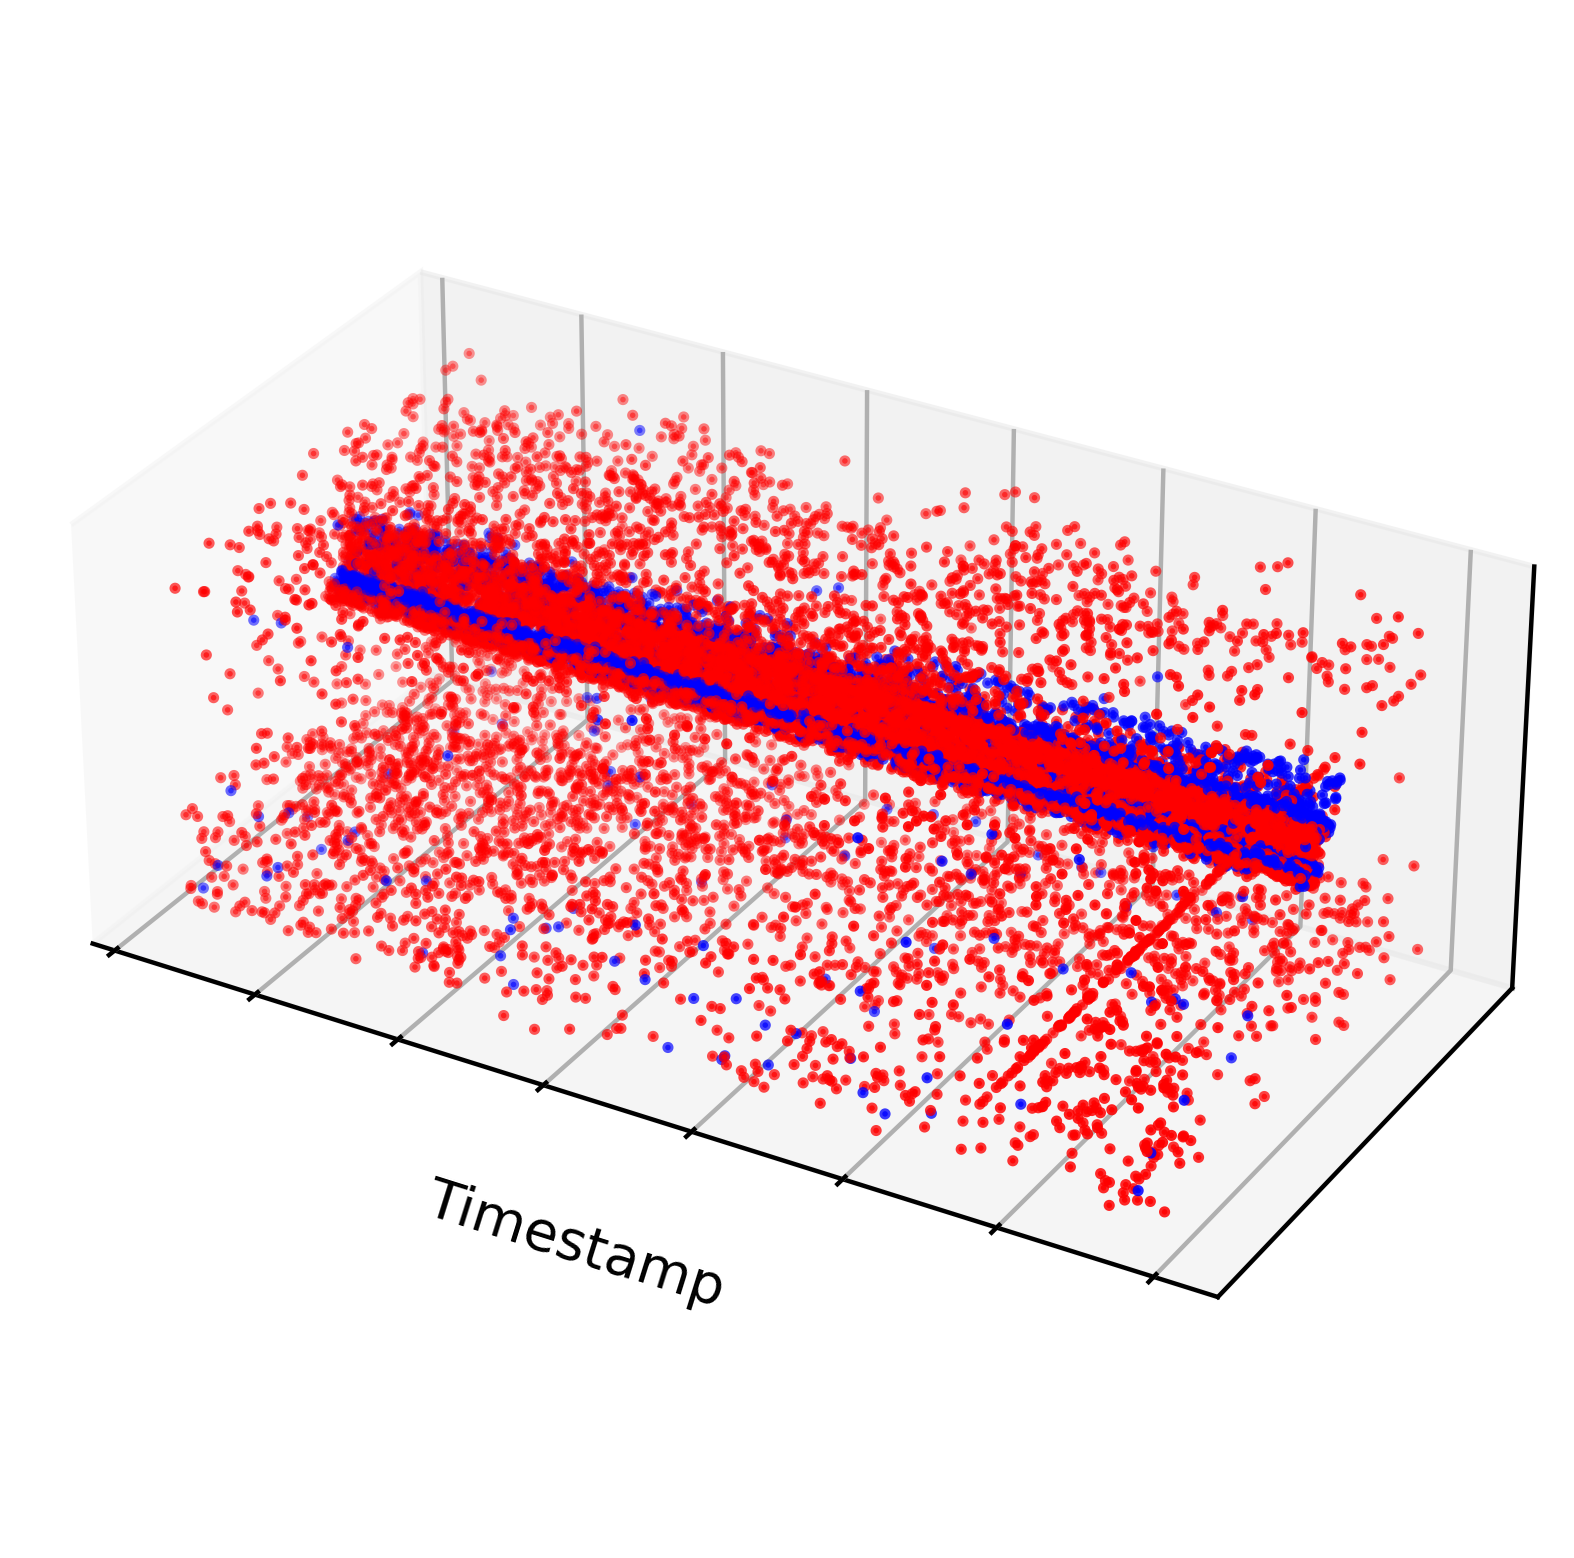
\includegraphics[width=\textwidth,trim=0 30 0 50,clip]{figures/dataset_denoising_01.png}
        \caption{去噪前}
    \end{subfigure}
    \hfill
    \begin{subfigure}{0.49\textwidth}
        \centering
        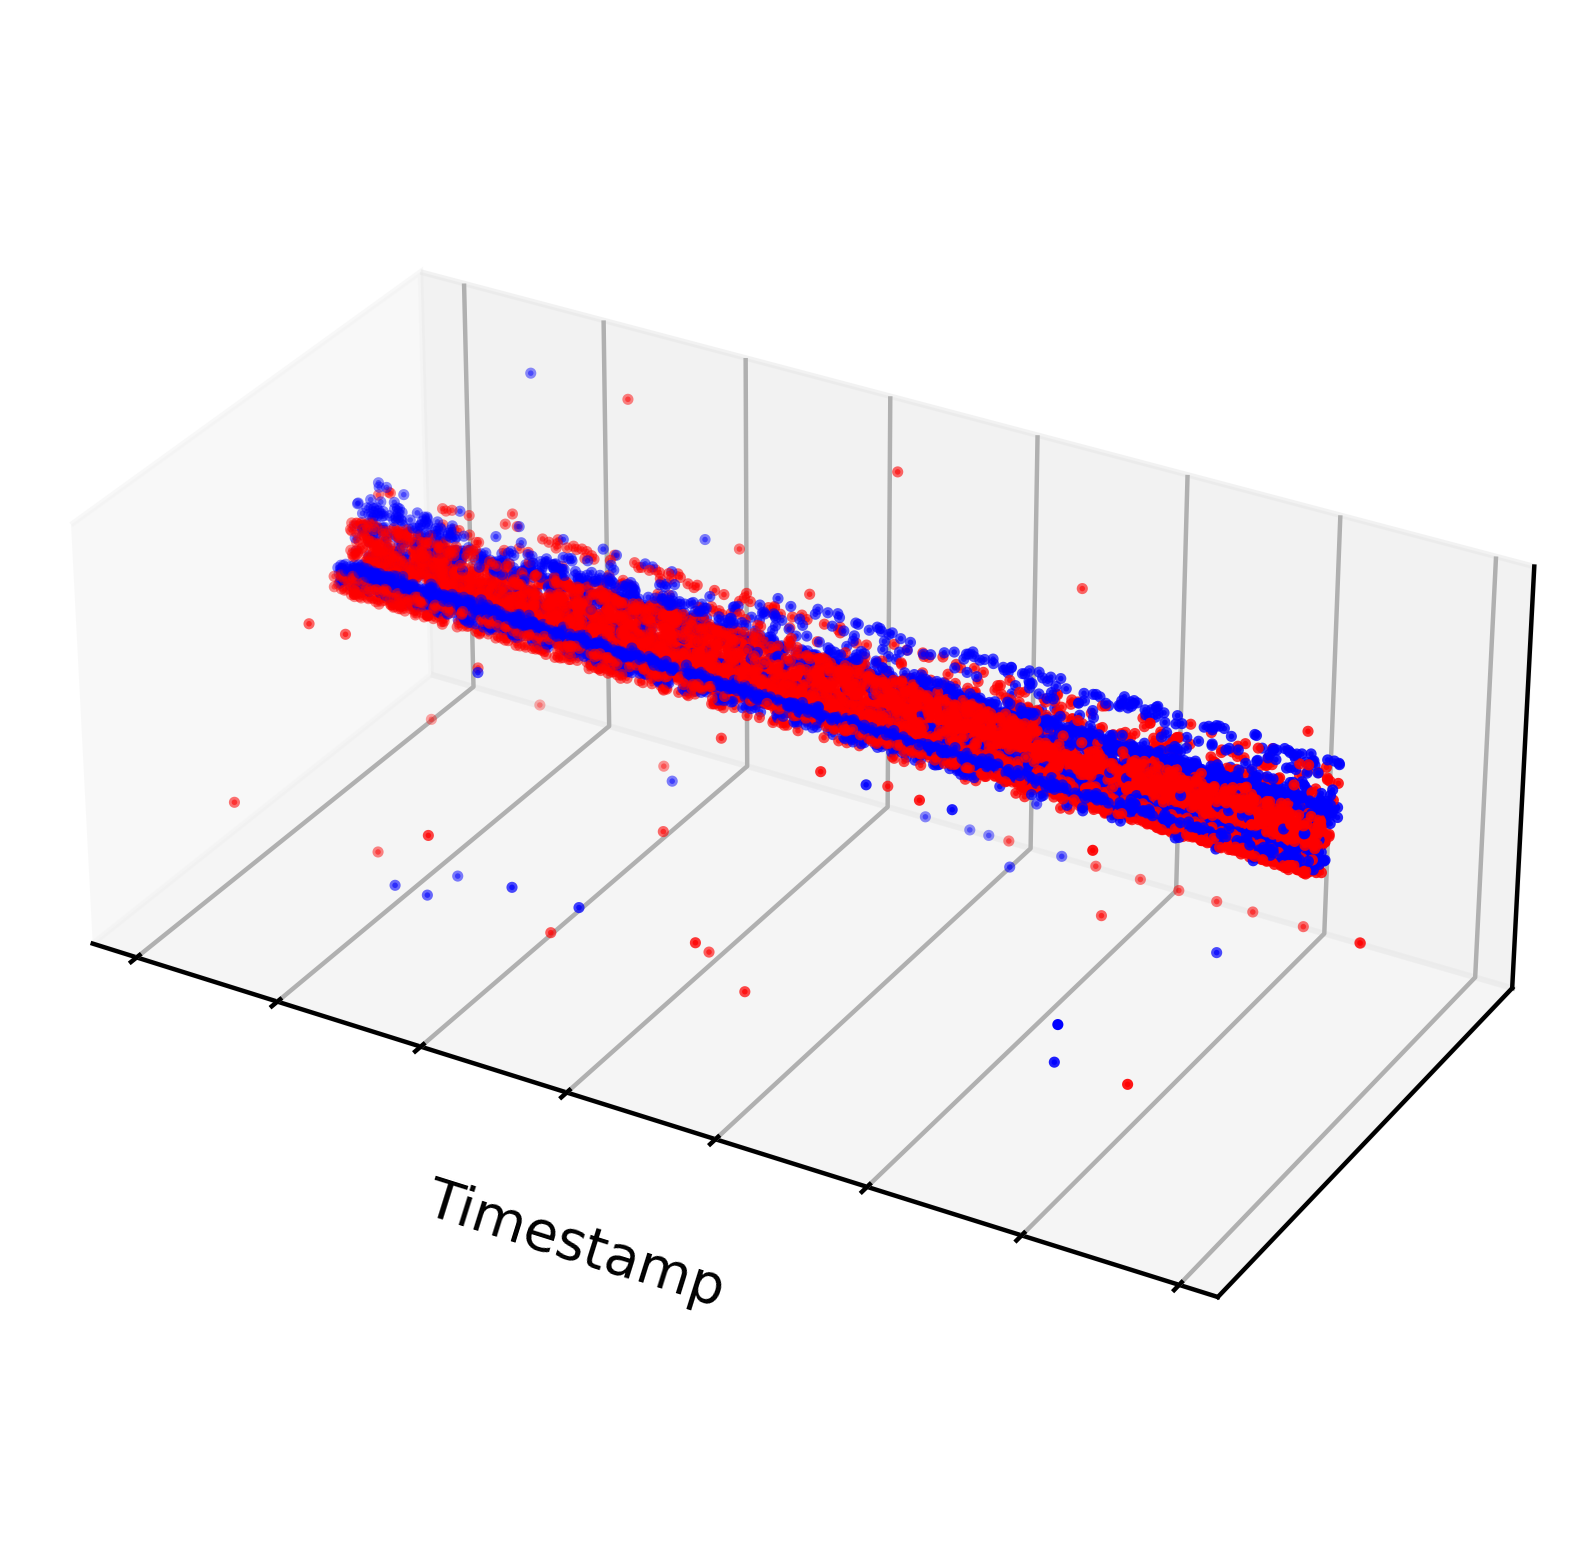
\includegraphics[width=\textwidth,trim=0 30 0 50,clip]{figures/dataset_denoising_02.png}
        \caption{去噪后}
    \end{subfigure}
    \caption{FlaDE数据集去噪处理}
    \label{subfig:FlaDE_denoising}
\end{figure}

步骤二:将事件投影为二进制事件图像(\ref{subfig:FlaDE_project_01})。这里参考\citet{kogler2009bio}提出的方法,将每组序列沿时间维度等间隔地进行切分,取$\Delta{t} \equiv \SI{33}{\milli\second}$,在同一时间间隔$\Delta{t}$内的事件被按坐标投影到相同分辨率的二维平面上,并按照极性构成由\{-1, 0, +1\}组成的二进制事件图像。

步骤三:融合二进制事件图像和灰度图像(\ref{subfig:FlaDE_project_02})。由于事件相机仅对运动物体产生响应,单纯的二进制事件图像可能会影响标定人员对运动物体类别的误判,因此需要引入灰度图像,以方便标定人员对场景进行确定。此处,本文通过计算同时间间隔内事件的时间平均,寻找到最近捕获的灰度图像,将两者按一定的权重进行融合,获得最终的标定图像。

\begin{figure}[ht]
    \centering
    \begin{subfigure}{0.49\textwidth}
        \centering
        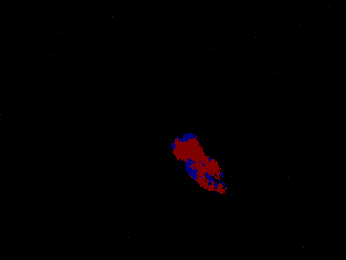
\includegraphics[width=\textwidth]{figures/dataset_project_01.png}
        \caption{事件投影}
        \label{subfig:FlaDE_project_01}
    \end{subfigure}
    \hfill
    \begin{subfigure}{0.49\textwidth}
        \centering
        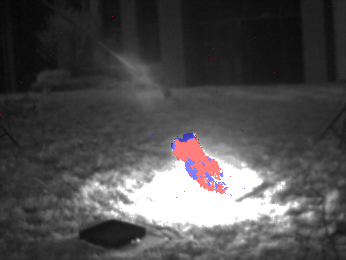
\includegraphics[width=\textwidth]{figures/dataset_project_02.png}
        \caption{融合灰度图像}
        \label{subfig:FlaDE_project_02}
    \end{subfigure}
    \caption{FlaDE数据集去噪处理}
\end{figure}

整个标定过程在CVAT\footnote{https://www.cvat.ai/}上进行,一个简单的标注示意如\ref{fig:annotation}所示。由专业人员逐帧手工标定完成,并且所有标签都会由另一位专业人员重新审核,最大限度地保证了数据集结果的可信度。

\begin{figure}
    \centering
    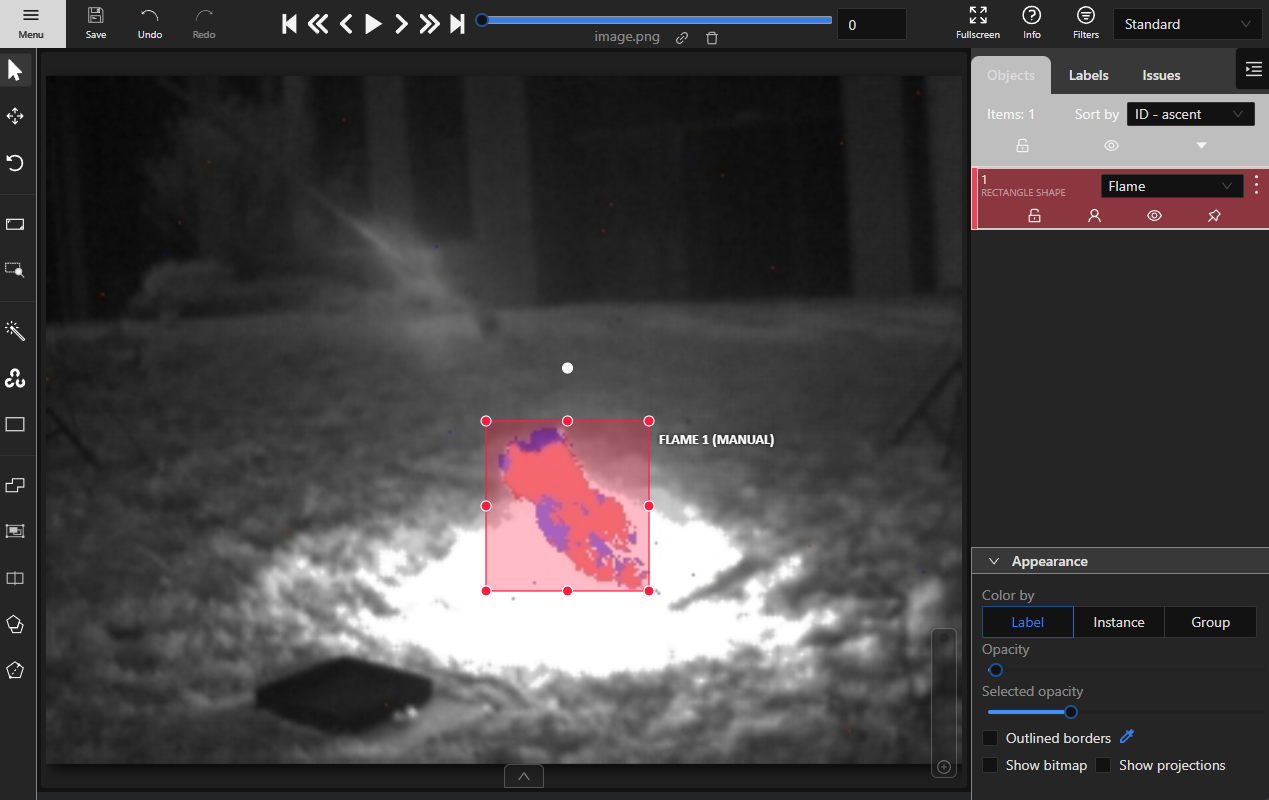
\includegraphics[width=0.9\textwidth]{figures/annotation.png}
    \caption{CVAT平台标注过程}
    \label{fig:annotation}
\end{figure}

\section{本章小结}
本章主要介绍了本文所使用的数据集的主要内容,制作过程与方法,后面的章节就会在这个FlaDE数据集基础上
进行提取特征工作以及检测算法构建工作。